\documentclass{article}
\usepackage[utf8]{inputenc}
\usepackage{graphicx,fancyhdr,amsmath,amssymb,amsthm,subfig,url,hyperref,enumerate}

% For payoff matrices
\usepackage{multirow,enumerate,array,float}
\usepackage[margin=1in]{geometry}

% For figures
\usepackage{graphicx}
\graphicspath{ {./figures/} }

\begin{document}
\title{Improving healthcare outcomes and cost through analysis and design of provider incentives}
\author{Keyan Pishdadian\\University of Washington\\\texttt{keyanp@cs.washington.edu}}
\date{March 2020}

\maketitle

\begin{abstract}
Provider decision making plays a critical role in patient outcomes and national healthcare spending. Creating robust incentive structures to underlie provider deicision making are vital to ensuring the delivery of high quality care and adequately managed costs. Despite this these incentive structures are poorly designed both financially and from a provider risk perspective. In this paper we analyze the inefficiencies and sub-optimal equilibria that result from the use of classic incentive systems, then extend recent ideas to propose a hybrid incentive structure that increases provider profits, improves patient outcomes, and reduces wasteful spending.
\end{abstract}


\section*{Introduction}

Healthcare is a socially and economically important aspect of the modern United States. Roughly 1/6th of US consumer spending \cite{econharvard} and ${\sim}48$\% of federal spending \cite{federalspend} goes towards some form of healthcare and the success, efficiency, and outcomes of this market reflect directly on the viability and happiness of American citizens and the US economy. The decision making of physicians plays a integral role in this system, with roughly 80\% of all expenditure being a result of physicians' decisions \cite{trust}. One becomes concerned with this control when comparing US healthcare expenditure to other developed countries (Fig. \ref{fig:usspend}), just why is expenditure so much higher in the US? At the root of the issue is that the healthcare market is unlike other normal markets where there is a buyer and a seller, with the buyer fully knowing what it is they want and having transparency into the price being offered by the seller \cite{msdt}. Rather, in this market there are many agents interacting directly or indirectly within a single healthcare transaction. We summarize these agents below\footnote{In order to simplify the model we ignore any altruistic behavior and moral incentives that we imagine (and hope) are present to some extent.}:

\begin{itemize}
    \item \textbf{patient}: who seeks to minimize cost to themselves, while maximizing quality of service
    \item \textbf{provider}: who seeks to maximize revenue to themselves, while minimizing volume of services rendered, and also minimizing financial and professional risk (e.g. malpratice lawsuits, increased cost of caring of patient with worsened condition)
    \item \textbf{hospital}: who seeks to maximize revenue, while minimizing cost and volume of service
    \item \textbf{other providers}: who act the same as the main provider, but whose actions have positive or negative externalities on the global wellbeing of the patient population
\end{itemize}

This results in a complex web of interdependencies between the agents (Fig. \ref{fig:agentdep}) which significantly complicates construction of effective incentive structures. Additionally the patient has little control in their outcomes aside from selecting a provider. In fact, the patient-provider relationship is a clear example of a \emph{principle-agent problem} \cite{principle} where the provider (the ``agent") must make diagnosis and care decisions that impact the patient (the ``principle"), but the provider/agent is motivated to act in their own best interests and not in the best interest of the patient/principle \cite{msdt}. Simultaneously, the provider is engaged in a game with other providers that closely resembles a ``prisoners' dilemmas", ultimately the decision making of any one provider has externalities on the health of the entire patient population, with a future decrease in overall health leading to an increase in the required volume of care to sustain proper health \cite{blended} affecting all providers.

In this paper we present each of the prevailing provider incentive structures, examine their benefits and inefficiencies, then use an adapted simplified model to formalize the resulting equilibria reached in each system. We briefly review the prisioners' dilemma model as a framework for analyzing provider decision making. We then extend recent ideas from Accountable Care Organizations (ACOs) to propose and analyze a hybrid incentive structure that increases provider profits and improves patient outcomes.

\begin{figure}[H]
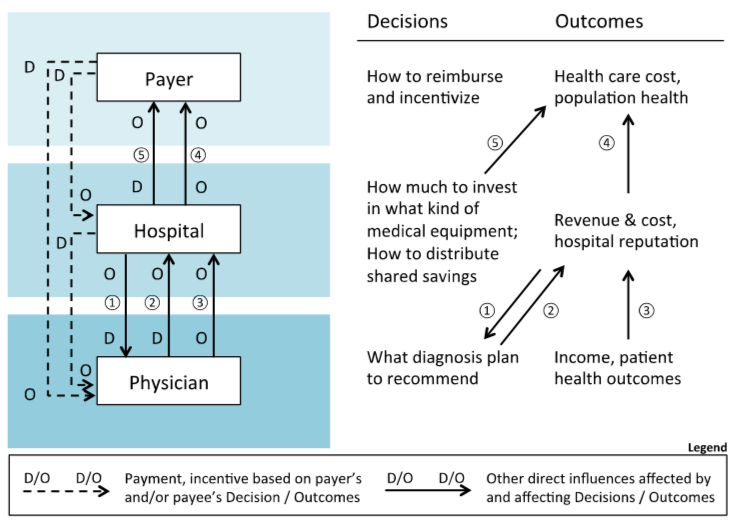
\includegraphics[height=7cm]{agentdep}
\centering
\caption{Agent interdepence diagram which shows the complex network of interactions between patients (Payer), providers (Physician), and hospitals. In this work we focus on controlling the decision making process (relations $1$ and $2$) and patient health outcomes and cost (relation $4$) \cite{msdt}.}
\label{fig:agentdep}
\end{figure}

\section*{Background}
In this section we review the two major incentive structures used for provider payment, \textbf{fee-for-service} and \textbf{capitation}. Discussion of the issues with each structure gives motivation to understanding the novel payment structure used by ACOs.

\subsection*{Fee-for-service}
This model is most familar to anyone who has interfaced with US healtcare. Here a provider is payed for each service rendered (e.g. surgery, office visit). Hence the payment to the provider is a direct function of the volume of services provided. Of course here the conflict of interest is clear that providers are incentivized to provide a high volume of low quality and high cost services, regardless of need. Aside from ethical considerations, the outcome of the patient has no bearing on the payoff of the provider. This observation is not surprising given the principle-agent backdrop coloring this relationship, and this has been documented an expectation of patients and other providers alike \cite{econharvard}\cite{overtreat}.

So what does this method get right? That same indifference to cost that begets high volume service may also allows access to expensive services that may give good results but have low probability of success. When providers do not fear increased spending then they are free to explore new treatment methods, equipment, medications, and procedures.

\subsection*{Capitation}
The capitation model is on the other end of the spectrum relative to fee-for-service models. Here a provider is paid a fixed sum for an agreed upon length of time for each patient that they oversee the health of. There are a wide range of methods used to compute capitation fees and payments structures that are outside the scope of this paper and discussed elsewhere, e.g. \cite{capfees}. Overall the principle is that providers want to reduce the number of services rendered and keep patients healthy so that they do no exceed the negotiated rate of payment per patient. Because any amount of spending beyond the negotiated capitation rate is entirely the responsbility of the provider/hospital, this model shifts significant risk to the provider to keep costs low, but has potential for greater financial payoff if the total cost of services rendered is significantly below the capitation fee.

Supporters of this model cite that it succeeds in reducing provider incentives to provide high volume services that are driven more by billing ability than by patient need \cite{blended}. However, there is fear that this design results instead in a low volume of low quality services. In fact it is this model that causes a prisioners' dilemma to arise between providers. Collectively all providers are better off if the health of the patient population in aggregate is good, as this means those patients will impose lower costs on each provider, but each provider's \emph{best response} strategy when making a care decision is ultimately to still provide low volume low quality care and free-ride on any provider that might be providing high volume high quality care. This point is formalized further in \textbf{Modeling Incentives}.

\subsection*{Accountable Care Organizations (ACOs)}
Foo bar baz

\section*{Modeling Incentives}
\label{section:modeling}

\subsection*{Prisioners' Dilemma}
For a thorough treatment of the prisoners' dilemma, refer to any number of game theory texts, e.g. \cite{networks}

\begin{table}[H]
\centering
  \setlength{\extrarowheight}{2pt}
  \begin{tabular}{*{4}{c|}}
    \multicolumn{2}{c}{} & \multicolumn{2}{c}{Prisioner II}\\\cline{3-4}
    \multicolumn{1}{c}{} &  & $S$  & $C$ \\\cline{2-4}
    \multirow{2}*{Prisioner I}  & $S$ & $(2,2)$ & $(12,1)$ \\\cline{2-4}
    & $C$ & $(1,12)$ & $(12,12)$ \\\cline{2-4}
  \end{tabular}
\caption{Payoff matrix zero-sum number calling game.}
\end{table}

\section*{Hybrid Approach}

%--------------------------------- Tables ----------------------------------


%--------------------------------- Figures ----------------------------------

\begin{figure}
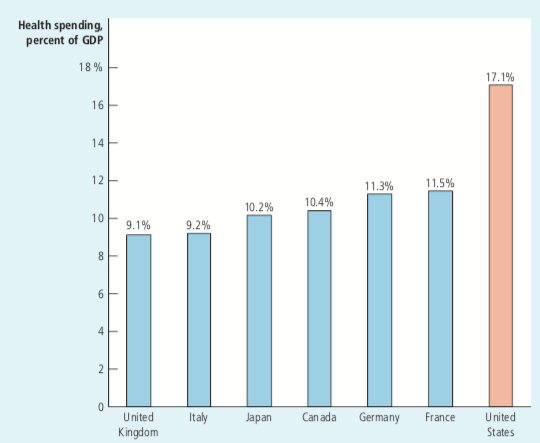
\includegraphics[height=7cm]{usspend}
\centering
\caption{US healthcare expenditure is significantly higher than that of other developed countries \cite{econharvard}.}
\label{fig:usspend}
\end{figure}

\begin{figure}
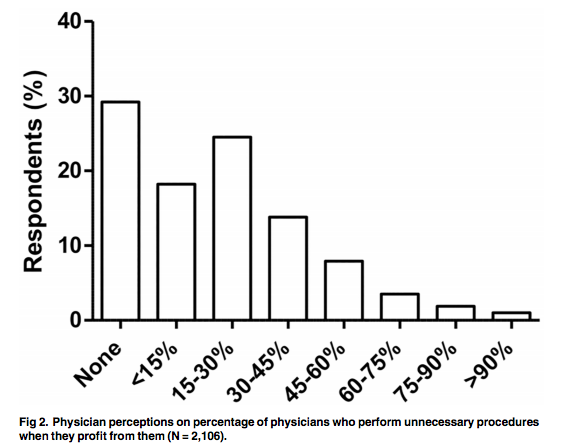
\includegraphics[height=7cm]{overtreat}
\centering
\caption{Provider responses when surveyed and asked what percentage of other physicians they think perform uneeded procedures financial gain \cite{overtreat}.}
\label{fig:overtreat}
\end{figure}

%--------------------------------- Bibliography ----------------------------------

\clearpage

\begin{thebibliography}{8}

\bibitem{federalspend}
The True Cost of Health Care: An Analysis of Americans’ Total Health Care Spend. https://bit.ly/39wbFzi

\bibitem{econharvard}
Mankiw NG. (2017) The Economics of Healthcare.

%6
\bibitem{trust}
Djulbegovic, Benjamin \& Hozo, Iztok \& Ioannidis, John. (2014). Modern health care as a game theory problem. European Journal of Clinical Investigation. 45. 10.1111/eci.12380

\bibitem{tim}
Roughgarden, T. (2016). Asymmetric Information and Reputation Systems. http://timroughgarden.org/f16/l/l12.pdf

\bibitem{overtreat}
Lyu H, Xu T, Brotman D, Mayer-Blackwell B, Cooper M, Daniel M, et al. (2017). Overtreatment in the United States. PLoS ONE 12(9): e0181970. https://doi.org/10.1371/journal.pone.0181970

% 1
% Cite as complicated approach by modifying how hospitals bill for services
\bibitem{inflation}
Agee, M.D., Gates, Z. (2013). Lessons from Game Theory about Healthcare System Price Inflation. Appl Health Econ Health Policy 11, 45–51. https://doi.org/10.1007/s40258-012-0003-z

%4
\bibitem{blended}
DeVoe, J. E., \& Stenger, R. (2013). Aligning provider incentives to improve primary healthcare delivery in the United States. OA family medicine, 1(1), 7. doi:10.13172/2052-8922-1-1-958

%5
\bibitem{msdt}
Zhang, H., Wernz, C. \& Slonim, A.D. (2016). Aligning incentives in health care: a multiscale decision theory approach. EURO J Decis Process 4, 219–244. https://doi.org/10.1007/s40070-015-0051-3

\bibitem{principle}
Eisenhardt, K. (1989). Agency Theory: An Assessment and Review. The Academy of Management Review, 14(1), 57-74. www.jstor.org/stable/258191

\bibitem{networks}
David, E., Kleinberg, J. (2010). Networks, Crowds, and Markets: Reasoning About a Highly Connected World. Cambridge University Press, USA. https://www.cs.cornell.edu/home/kleinber/networks-book/

\bibitem{acos}
Redding, K. (2018). Participation and Performance in Accountable Care Organizations, Doctoral Disertation.

\bibitem{capfees}
Iezzoni, Lisa I. et al. (1998). Paying More Fairly for Medicare Capitated Care. New England Journal of Medicine. https://doi.org/10.1056/NEJM199812243392613

\end{thebibliography}

%-------------------------------------------------------------------

\end{document}
